%% LyX 2.0.2 created this file.  For more info, see http://www.lyx.org/.
%% Do not edit unless you really know what you are doing.
\documentclass[a4paper,english]{article}
\usepackage[latin9]{inputenc}
\usepackage{color}
\usepackage{array}
\usepackage{textcomp}
\usepackage{multirow}
\usepackage{amsmath}
\usepackage{amssymb}
\usepackage{graphicx}
\usepackage{esint}

\makeatletter

%%%%%%%%%%%%%%%%%%%%%%%%%%%%%% LyX specific LaTeX commands.
\special{papersize=\the\paperwidth,\the\paperheight}

%% Because html converters don't know tabularnewline
\providecommand{\tabularnewline}{\\}

%%%%%%%%%%%%%%%%%%%%%%%%%%%%%% User specified LaTeX commands.

\usepackage{interspeech2013}\usepackage{epsfig}\setcounter{page}{1}
\sloppy	
\ninept
\def\reg{{\rm\ooalign{\hfil
     \raise.07ex\hbox{\scriptsize R}\hfil\crcr\mathhexbox20D}}}



\usepackage{babel}





\usepackage{babel}

\makeatother

\usepackage{babel}
\begin{document}

\title{Comparison of approaches for an efficient phonetic decoding}

\maketitle
\makeatletter \makeatother 
\begin{abstract}
This article analyzes the phonetic decoding performance obtained with
different choices of linguistic units. The context is to later use
such an approach as a support for helping communication with deaf
people, and to run it on an embedded decoder on a portable terminal,
which introduces constrains on the model size. As a first step, this
paper presents and analyses the performance of various approaches.
Two baseline systems are considered, one relying on a large vocabulary
speech recognizer, and another one relying on a phonetic n-gram language
model. Then syllable-based lexicons and language models are investigated.
Various lexicon sizes are studied by setting thresholds on their frequency
of occurrences in the training data. Evaluations are conducted on
the ESTER and ETAPE speech corpora. Keeping only the most frequent
syllables leads to a limited-size lexicon and language model, which
nevertheless provides good phonetic decoding performance. The phone
error rate is only 4\% worse (absolute) than the phone error rate
obtained with the large vocabulary recognizer, and much better than
the phone error rate obtained with the phone n-gram language model.
\end{abstract}
\noindent \textbf{Index Terms}: phonemes, syllables, deaf, speech
recognition, embedded system.


\section{Introduction}

Support for deaf people or for people with hearing impairment is an
application area of automatic speech processing technologies \cite{IS1}.
Their objective is to become a communication aid for disabled persons,
to insure a better comprehension for the user (by the means of speech
recognition) and also a better communication from the user (by the
means of speech synthesis).

Over the past decades, scientists have tried to offer a better speech
understanding, by displaying phonetic features to help lipreading
\cite{IS2}, by displaying signs in sign language through an avatar
\cite{IS3}, and of course by displaying subtitles, generated in a
semi-automatic or fully automatic manner. The ergonomic aspects and
the conditions for using speech recognition to help deaf people were
analyzed in \cite{IS4}.

One of the main drawbacks of speech recognition systems is their incapacity
of recognizing the words that do not belong to their vocabulary. Given
the limited amount of speech training data, and also the need of a
compromise between a reasonable memory use and a reasonable recognizer's
performance with an acceptable execution time, it is impossible to
conceive a system that covers all the words, let alone the proper
names or abbreviations. When a spoken word can not be identified within
the current vocabulary, the recognition system will automatically
recognize it as an other one close to it, or as a series of other
small words acoustically similar to the unknown word. Furthermore,
recognition systems are not perfect, it happens quite frequently that
a word is confused with another one which is pronounced the same (homophone)
or almost the same. The performances are very far from human performance
\cite{IS5} and even degrade rapidly in the presence of noise. Therefore,
in the context of communication aids for deaf people, displaying the
orthographic form of the recognized words may not be an ideal solution.

IBM has thus tested subtitling the phonetic speech of a speaker, with
the system called LIPCOM \cite{IS6}. The recognition system was mono-speaker,
and has been tested in a school for deaf children. The application
was based on a phonetic decoding (with no prior defined vocabulary)
and the result was displayed as phonemes coded on one or two letters.
More recent studies have measured the contribution of confidence measures
\cite{IS7} within the use of automatic transcription for deaf people
\cite{IS8}. Subjective tests have shown a preference for displaying
the phonetic form of the words with a low confidence score.

An alternative solution is to use multi-phone sub-word units, like
the syllable. Its appeal lies in its close connection to human speech
perception and articulation, since it's more intuitive for representing
speech sounds. In fact, the syllable is a unit longer than the phoneme,
easier to index and offers the possibility of generating an unlimited
number of words with only a few thousands of basic items. The use
of syllable-size acoustic units in speech recognition has been investigated
in the past \cite{IS9,IS10}, for large vocabulary continuous speech
recognition (usually in combination with context dependent phones)
\cite{IS11,IS12} or for phonetic decoding only \cite{IS13}. In this
last case \cite{IS13}, because of the structure of the acoustic units,
coarticulation was modeled between phonemes inside the syllable unit,
but no context-dependent modeling was taken into account between syllable
units, moreover the language model applied at the syllable level was
a bigram. Besides, to overcome the limited size of any speech recognizer
lexicon, studies have been conducted in extending the word-based lexicon
with fragments, typically sequences of phonemes determined in a data
driven way; this extension helps providing better acoustic matches
on out-of-vocabulary portions of the speech signal, which globally
leads to a smaller phonetic error rate \cite{IS14}. 

In this paper we shall investigate the use of syllables at the lexical
level. The pronunciation of the syllables are described in terms of
phonemes, which are modeled with context-dependent 3-states HMM. The
language model applied on the syllables is a trigram. We have followed
the rules proposed in a recent study for detecting syllables boundaries
within a sequence of phonemes \cite{IS15}. These rules are used to
derive the syllables from the phonetic forced-aligned training data,
and some criteria are applied to reduce the list of syllables constituting
the lexicon. Performance is reported in terms of phoneme error rate,
and evaluations are conducted on two large French speech corpus.

\begin{figure*}
\begin{centering}
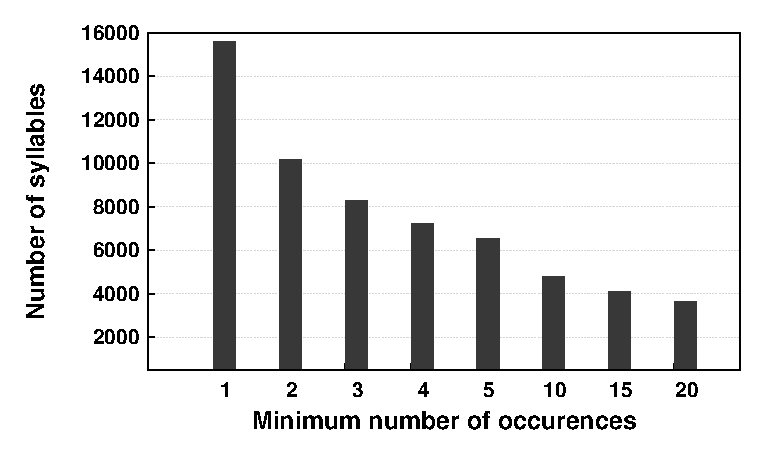
\includegraphics[scale=0.63]{Image/syllables_minocc}\hspace{0.2cm}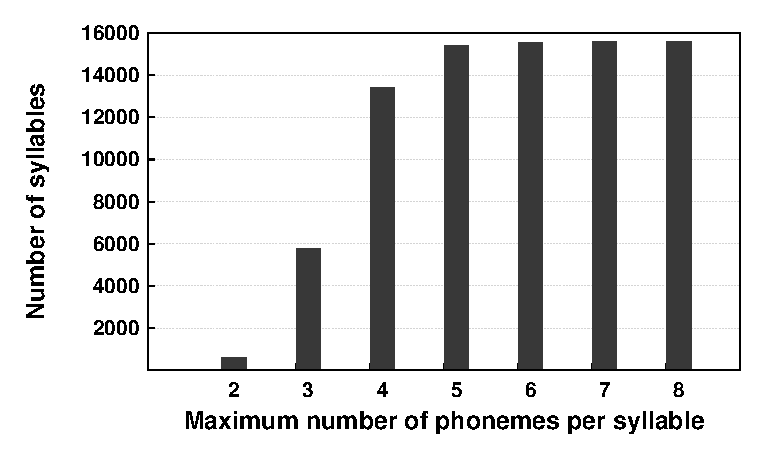
\includegraphics[scale=0.63]{Image/syllables_maxph}
\par\end{centering}

\caption{Number of syllables with respect to the minimum number of occurrences
(left) and maximum number of phonemes per syllable (right)}
\label{Fig:syllables}
\end{figure*}


The work presented in this paper is part of the RAPSODIE project,
which aims at studying, deepening and richening the extraction of
relevant speech information, in order to support communication with
deaf or hard of hearing people. Therefore, the optimal solution should
determine the best compromise for the recognition model and the best
way of presenting the recognized information (words, syllables, phonemes
or combinations), within the constraints of limited available resources
(the memory size and computational power of an embedded system). 

This article thus performs a detailed study and analysis of the performance
of various modules (in particular the choice of linguistic units and
their associated language model) and heuristic decoding to obtain
the best compromise between computational cost and usability results.
The first section provides a description of the various linguistic
units used in our analysis. The second part of the paper is devoted
to the description of experiments and the discussion of results.


\section{Choice of linguistic units}

This section describes the linguistic units used in our analysis:
the phonemes, as the basic and smallest linguistic unit, the syllables,
as the phonological ``building blocks'' of words, and the words,
as the largest linguistic unit, but at the same time the smallest
linguistic element which caries a real meaning.

Note that the choice of linguistic units impacts on the choice of
the vocabulary and of the language model. In the experiments reported
later, the acoustic unit will always be the phoneme. 

The language models used in our analysis are trigram statistical models,
thus for each three lexical unit sequence, the probability of the
last unit depends on the identity of the two units that precede it. 


\subsection{Phonemes}

Regarding the pronunciation lexicon, the pronunciation of a phoneme
is the phoneme itself. 

Using this type of linguistic unit, we minimize the size of our vocabulary
(less than 40 phonemes for the French language) and therefore the
size of our language model. But unfortunately, with less modeling
power usually comes worse performance. 


\subsection{Words}

The words vocabulary contains the mappings from words to their pronunciations
in the given phoneme set. Part of the reason why French pronunciation
is so difficult is due to the fact that French is a non-phonetic language
(some letters can be pronounced in different ways or sometimes not
at all) and to ``liaisons''. A liaison is the phenomenon whereby
a normally silent consonant at the end of a word is pronounced at
the beginning of the word that follows it. So, in order to make the
automatic phonetic transcription as fluid as the real speech (and
thus mimic real pronunciations), scientist usually consider within
the dictionary all possible ``liaison'' events between words. Like
for example, in the sentence ``les oiseaux'', a classical word to
phoneme transcription would give ``l eh w a z o'', instead of returning
the real pronunciation ``l eh z w a z o''.

Using this type of linguistic unit leads to a large vocabulary (about
97,000 words in our dictionary) and therefore also to a large language
model.\textcolor{black}{{} This kind of model usually gives the best
performance, but with the cost of great memory use and slow computational
time (not ideal for embedded systems).}


\subsection{Syllables}

Regarding the vocabulary, the pronunciation of a syllable (phonetic
in our case) is its decomposition into the phonemic components. 

In order to account for the ``liaison'' events, the words will not
be processed individually. The training corpora is entirely phonetized
and the resulting continuous list of phonemes will be processed by
the syllabification tool. The phonetization process is realized by
force-aligning the manual transcriptions; each word is then replaced
with its corresponding pronunciation variant found in the words vocabulary.
Note that the vocabularies used in speech recognition follow real
pronunciations, which means that a word can have several pronunciation
variants, and that one or more phonemes might be missing in some of
them. 

\begin{figure*}
\begin{centering}
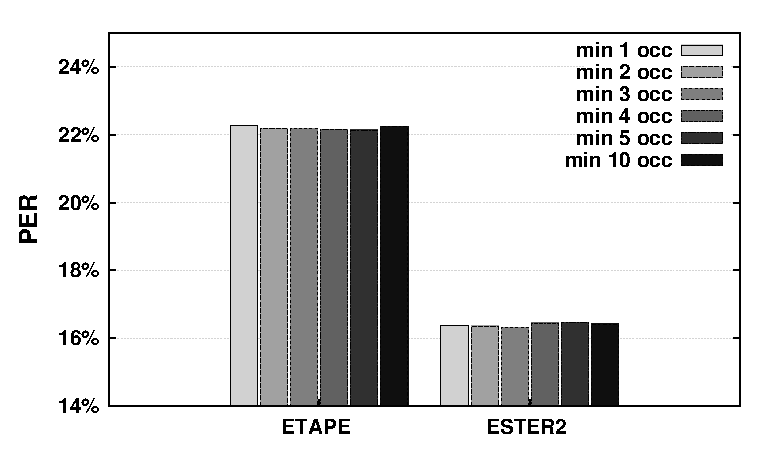
\includegraphics[scale=0.63]{Image/results_minocc}\hspace{0.2cm}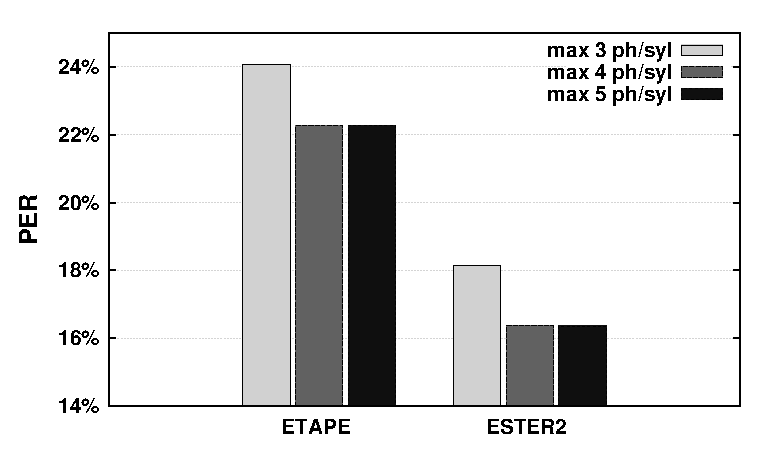
\includegraphics[scale=0.63]{Image/results_maxph}
\par\end{centering}

\caption{Performance analysis on the syllabic n-gram language models, selected
according to a minimum number of occurrences (left) or to a maximum
number of phonemes per syllable (right)}
\label{Fig:Perform_min_max}
\end{figure*}


Our syllabification tool is based on the rules described in \cite{IS15},
which follow two main principles: a syllable contains a single vowel
and a pause designates a syllable's boundary. Therefore, the syllabification
algorithm will give out models of syllables and pseudo-syllables.
The pseudo-syllables are the units where one vowel is surrounded by
a great number of consonants, which normally shouldn't belong to a
single syllable. Using this kind of models is acceptable in automatic
transcriptions , because it is quite frequent that users ``skip''
phonemes in their fluid, fast pronunciations ans also that is quite
frequent that recognition systems ``skip'' too short, non-obvious
phonemes. We have tried to reduce the number of abnormally-long pseudo-syllables
(those that cover more than 2 words) by using as additional information
the boundaries between words, but the results were not improved.

In order to filter some of the pseudo-syllable models, we have chosen
to create different lists corresponding to two criteria : a minimum
number of occurrences within the training corpora, and a maximum number
of phonemes per syllable. Figure \ref{Fig:syllables} presents the
number of syllables resulting from the application of each criterion
(the used corpora is described in section \ref{sub:Data}).

Using syllables as linguistic units leads to a compromise between
the memory use (up to 16000 syllables within our dictionary) and\textcolor{black}{{}
computational time (ideal for embedded systems).}


\section{Experiments and results}

This section describes the data sets and tools used in our experiments,
along with the corresponding results.


\subsection{Data\label{sub:Data}}

The speech corpora used in our experiments come from the ESTER2 \cite{IS17}
and the ETAPE \cite{IS18} evaluation campaigns, and the EPAC \cite{IS19}
project. The ESTER2 and EPAC data are French broadcast news collected
from various radio channels, thus they contain prepared speech, plus
interviews. A large part of the speech data is of studio quality,
and some parts are of telephone quality. On the opposite, the ETAPE
data correspond to debates collected from various radio and TV channels.
Thus this is mainly spontaneous speech. 

The speech data of the ESTER2 and ETAPE train sets, as well as the
transcribed data from the EPAC corpus, were used to train the acoustic
models. The training data amounts to almost 300 hours of signal and
almost 4 million running words. The phoneme-based language model and
the syllable-based language models were also trained on the ESTER2,
ETAPE and EPAC text corpora, on about 12 million running phonemes
and on about 6 million running syllables.

For the creation of the word-based language model, various text corpora
were used: more than 500 million words of newspaper data from 1987
to 2007; several million words from transcriptions of various radio
broadcast shows; more than 800 million words from the French Gigaword
corpus \cite{IS20} from 1994 to 2008; plus 300 million words of web
data collected in 2011 from various web sources, and thus mainly covering
recent years. 

For the word-based lexicon, the vocabulary of about 97,000 words,
was developed for the ETAPE evaluation campaign. The pronunciation
variants were extracted from the BDLEX lexicon \cite{IS21} and from
in-house pronunciation lexicons, when available. For the missing words,
the pronunciation variants were automatically obtained using JMM-based
and CRF-based Grapheme-to-Phoneme converters \cite{IS22}. 


\subsection{Configuration}

The SRILM tools \cite{IS23} were used to create the statistical language
models. 

The Sphinx3 tools \cite{IS24} were used to convert the SRILM language
models into the Sphinx3 format and to decode the audio signals. 

The MFCC (Mel Frequency Cepstral Coefficients) acoustic analysis gives
12 MFCC parameters and a logarithmic energy per frame (window of 32
ms, 10 ms shift).

The acoustic HMM models were modeled with a 64 Gaussian mixture, and
adapted to male and female data. 


\subsection{Results}

The development sets of the ESTER2 (non-African radios, about 42,000
running words) and ETAPE (entire set, about 82,000 running words)
data are used in the experiments reported below. 

\begin{table}[h]
\begin{centering}
\begin{tabular}{|>{\raggedright}p{1.55cm}|r@{\extracolsep{0pt}.}l|r@{\extracolsep{0pt}.}l|r@{\extracolsep{0pt}.}l|r@{\extracolsep{0pt}.}l|}
\hline 
\multirow{2}{1.55cm}{\textbf{\textcolor{black}{LM}}} & \multicolumn{6}{c|}{\textbf{\# of }\textbf{\textit{n}}\textbf{-grams}} & \multicolumn{2}{>{\centering}p{0.9cm}|}{\textbf{Size}}\tabularnewline
\cline{2-7} 
 & \multicolumn{2}{c|}{\textbf{n=1}} & \multicolumn{2}{c|}{\textbf{n=2}} & \multicolumn{2}{c|}{\textbf{n=3}} & \multicolumn{2}{c|}{\textbf{{[}MB{]}}}\tabularnewline
\hline 
\hline 
\textcolor{black}{phonemes} & \multicolumn{2}{c|}{40} & \multicolumn{2}{c|}{1347} & \multicolumn{2}{c|}{30898} & 0&21\tabularnewline
\hline 
\hline 
\textcolor{black}{syl\_min1occ} & 15&6 K & 0&38 M & 1&74 M & 10&28\tabularnewline
\hline 
\textcolor{black}{syl\_min2occ} & 10&2 K & 0&38 M & 1&73 M & 10&07\tabularnewline
\hline 
\textcolor{black}{syl\_min3occ} & 8&3 K & 0&38 M & 1&73 M & 9&97\tabularnewline
\hline 
\textcolor{black}{syl\_min4occ} & 7&2 K & 0&37 M & 1&73 M & 9&90\tabularnewline
\hline 
\textcolor{black}{syl\_min5occ} & 6&5 K & 0&36 M & 1&73 M & 9&85\tabularnewline
\hline 
\textcolor{black}{syl\_min10occ} & 4&8 K & 0&35 M & 1&71 M & 9&65\tabularnewline
\hline 
\hline 
\textcolor{black}{syl\_max3ph} & 5&8 K & 0&29 M & 1&56 M & 8&60\tabularnewline
\hline 
\textcolor{black}{syl\_max4ph} & 13&4 K & 0&38 M & 1&73 M & 10&14\tabularnewline
\hline 
\textcolor{black}{syl\_max5ph} & 15&4 K & 0&38 M & 1&74 M & 10&27\tabularnewline
\hline 
\hline 
words & 97&3 K & 43&35 M & 79&30 M & 1269&81\tabularnewline
\hline 
\end{tabular}
\par\end{centering}

\caption{The description of language models}
\label{Tab:LMs}
\end{table}


The COALT (Comparing Automatic Labelling Tools) software \cite{IS25}
was used for the analysis of results (phoneme error rates). The compared
files are the hypothesis .ctm file (resulting from the decoding process)
along with the reference .stm file. The CTM file consists of a concatenation
of time-marked phonemes. The STM (segment time marked) file describes
the reference transcript and consists of a concatenation of text segments.
We forced-aligned the STM files, in order for them to contain concatenations
of time-marked phonemes as well.

Table \ref{Tab:LMs} describes the language models used in our experiments.
With phoneme-based units, the number of 3-grams is around 30,000 which
leads to a minimum disk usage. With different lists of syllables,
the number of 3-grams is around 1,700,000 which leads to an average
disk usage. Using a large vocabulary, the number of 3-grams is around
79,000,000 which leads to the largest disk usages.

\begin{table}[h]
\begin{centering}
\begin{tabular}{|>{\raggedright}p{1.55cm}|r@{\extracolsep{0pt}.}l|r@{\extracolsep{0pt}.}l|r@{\extracolsep{0pt}.}l|r@{\extracolsep{0pt}.}l|}
\hline 
\multirow{1}{1.55cm}{\textbf{LM}} & \multicolumn{2}{c|}{\textbf{PER}} & \multicolumn{2}{c|}{\textbf{Ins}} & \multicolumn{2}{c|}{\textbf{Del}} & \multicolumn{2}{c|}{\textbf{Sub}}\tabularnewline
\hline 
\hline 
\textcolor{black}{phonemes} & \textcolor{black}{38}&\textcolor{black}{22} & \textcolor{black}{2}&\textcolor{black}{87} & \textcolor{black}{15}&\textcolor{black}{41} & \textcolor{black}{19}&\textcolor{black}{94}\tabularnewline
\hline 
\hline 
\textcolor{black}{syl\_min1occ} & \textcolor{black}{22}&\textcolor{black}{26} & \textcolor{black}{3}&\textcolor{black}{37} & \textcolor{black}{8}&\textcolor{black}{64} & \textcolor{black}{10}&\textcolor{black}{25}\tabularnewline
\hline 
\textcolor{black}{syl\_min2occ} & \textcolor{black}{22}&\textcolor{black}{19} & \textcolor{black}{3}&\textcolor{black}{36} & \textcolor{black}{8}&\textcolor{black}{63} & \textcolor{black}{10}&\textcolor{black}{20}\tabularnewline
\hline 
\textcolor{black}{syl\_min3occ} & \textcolor{black}{22}&\textcolor{black}{18} & \textcolor{black}{3}&\textcolor{black}{37} & \textcolor{black}{8}&\textcolor{black}{62} & \textcolor{black}{10}&\textcolor{black}{19}\tabularnewline
\hline 
\textcolor{black}{syl\_min4occ} & \textcolor{black}{22}&\textcolor{black}{16} & \textcolor{black}{3}&\textcolor{black}{36} & \textcolor{black}{8}&\textcolor{black}{62} & \textcolor{black}{10}&\textcolor{black}{18}\tabularnewline
\hline 
\textbf{\textcolor{black}{syl\_min5occ}} & \textbf{\textcolor{black}{22}}&\textbf{\textcolor{black}{14}} & \textbf{\textcolor{black}{3}}&\textbf{\textcolor{black}{35}} & \textbf{\textcolor{black}{8}}&\textbf{\textcolor{black}{60}} & \textbf{\textcolor{black}{10}}&\textbf{\textcolor{black}{19}}\tabularnewline
\hline 
\textcolor{black}{syl\_min10occ} & \textcolor{black}{22}&\textcolor{black}{24} & \textcolor{black}{3}&\textcolor{black}{37} & \textcolor{black}{8}&\textcolor{black}{63} & \textcolor{black}{10}&\textcolor{black}{23}\tabularnewline
\hline 
\hline 
\textcolor{black}{syl\_max3ph} & \textcolor{black}{24}&\textcolor{black}{06} & \textcolor{black}{3}&\textcolor{black}{63} & \textcolor{black}{9}&\textcolor{black}{34} & \textcolor{black}{11}&\textcolor{black}{10}\tabularnewline
\hline 
\textcolor{black}{syl\_max4ph} & \textcolor{black}{22}&\textcolor{black}{26} & \textcolor{black}{3}&\textcolor{black}{37} & \textcolor{black}{8}&\textcolor{black}{65} & \textcolor{black}{10}&\textcolor{black}{25}\tabularnewline
\hline 
\textcolor{black}{syl\_max5ph} & \textcolor{black}{22}&\textcolor{black}{28} & \textcolor{black}{3}&\textcolor{black}{37} & \textcolor{black}{8}&\textcolor{black}{64} & \textcolor{black}{10}&\textcolor{black}{26}\tabularnewline
\hline 
\hline 
\textbf{\textcolor{black}{words}} & \textbf{\textcolor{black}{18}}&\textbf{\textcolor{black}{36}} & \textbf{\textcolor{black}{3}}&\textbf{\textcolor{black}{14}} & \textbf{\textcolor{black}{8}}&\textbf{\textcolor{black}{16}} & \textbf{\textcolor{black}{7}}&\textbf{\textcolor{black}{06}}\tabularnewline
\hline 
\end{tabular}
\par\end{centering}

\caption{Performance analysis on ETAPE corpora {[}\%{]}}
\label{Tab:performance-ETAPE}
\end{table}


Table \ref{Tab:performance-ETAPE} presents the results obtained on
the ETAPE's development set. As expected, the best results were obtained
with the large vocabulary recognizer. By using only the most frequent
syllables within the language model, we limit the size of the lexicon
( about 7000 syllables, cf. Figure \ref{Fig:syllables} ) and the
size of the language model (only about 10MB, cf. Table \ref{Tab:LMs}),
and we achieve nevertheless good phonetic decoding performances. The
phone error rate is only 4\% worse (absolute) than the phone error
rate obtained with the large vocabulary recognizer, and much better
than the phone error rate obtained with the phone n-gram language
model.

\begin{table}[h]
\begin{centering}
\begin{tabular}{|>{\raggedright}p{1.55cm}|r@{\extracolsep{0pt}.}l|r@{\extracolsep{0pt}.}l|r@{\extracolsep{0pt}.}l|r@{\extracolsep{0pt}.}l|}
\hline 
\multirow{1}{1.55cm}{\textbf{LM}} & \multicolumn{2}{c|}{\textbf{PER}} & \multicolumn{2}{c|}{\textbf{Ins}} & \multicolumn{2}{c|}{\textbf{Del}} & \multicolumn{2}{c|}{\textbf{Sub}}\tabularnewline
\hline 
\hline 
\textcolor{black}{phonemes} & \textcolor{black}{34}&\textcolor{black}{24} & \textcolor{black}{3}&\textcolor{black}{66} & \textcolor{black}{11}&\textcolor{black}{62} & \textcolor{black}{18}&\textcolor{black}{97}\tabularnewline
\hline 
\hline 
\textcolor{black}{syl\_min1occ} & \textcolor{black}{16}&\textcolor{black}{38} & \textcolor{black}{4}&\textcolor{black}{05} & \textcolor{black}{5}&\textcolor{black}{05} & \textcolor{black}{7}&\textcolor{black}{28}\tabularnewline
\hline 
\textcolor{black}{syl\_min2occ} & \textcolor{black}{16}&\textcolor{black}{36} & \textcolor{black}{4}&\textcolor{black}{05} & \textcolor{black}{5}&\textcolor{black}{05} & \textcolor{black}{7}&\textcolor{black}{26}\tabularnewline
\hline 
\textbf{\textcolor{black}{syl\_min3occ}} & \textbf{\textcolor{black}{16}}&\textbf{\textcolor{black}{33}} & \textbf{\textcolor{black}{4}}&\textbf{\textcolor{black}{04}} & \textbf{\textcolor{black}{5}}&\textbf{\textcolor{black}{06}} & \textbf{\textcolor{black}{7}}&\textbf{\textcolor{black}{23}}\tabularnewline
\hline 
\textcolor{black}{syl\_min4occ} & \textcolor{black}{16}&\textcolor{black}{45} & \textcolor{black}{4}&\textcolor{black}{06} & \textcolor{black}{5}&\textcolor{black}{05} & \textcolor{black}{7}&\textcolor{black}{34}\tabularnewline
\hline 
\textcolor{black}{syl\_min5occ} & \textcolor{black}{16}&\textcolor{black}{47} & \textcolor{black}{4}&\textcolor{black}{04} & \textcolor{black}{5}&\textcolor{black}{06} & \textcolor{black}{7}&\textcolor{black}{36}\tabularnewline
\hline 
\textcolor{black}{syl\_min10occ} & \textcolor{black}{16}&\textcolor{black}{42} & \textcolor{black}{4}&\textcolor{black}{00} & \textcolor{black}{5}&\textcolor{black}{10} & \textcolor{black}{7}&\textcolor{black}{32}\tabularnewline
\hline 
\hline 
\textcolor{black}{syl\_max3ph} & \textcolor{black}{18}&\textcolor{black}{15} & \textcolor{black}{4}&\textcolor{black}{37} & \textcolor{black}{5}&\textcolor{black}{67} & \textcolor{black}{8}&\textcolor{black}{11}\tabularnewline
\hline 
\textcolor{black}{syl\_max4ph} & \textcolor{black}{16}&\textcolor{black}{37} & \textcolor{black}{4}&\textcolor{black}{02} & \textcolor{black}{5}&\textcolor{black}{07} & \textcolor{black}{7}&\textcolor{black}{27}\tabularnewline
\hline 
\textcolor{black}{syl\_max5ph} & \textcolor{black}{16}&\textcolor{black}{36} & \textcolor{black}{4}&\textcolor{black}{04} & \textcolor{black}{5}&\textcolor{black}{04} & \textcolor{black}{7}&\textcolor{black}{28}\tabularnewline
\hline 
\hline 
\textbf{\textcolor{black}{words}} & \textbf{\textcolor{black}{12}}&\textbf{\textcolor{black}{76}} & \textbf{\textcolor{black}{3}}&\textbf{\textcolor{black}{52}} & \textbf{\textcolor{black}{4}}&\textbf{\textcolor{black}{84}} & \textbf{\textcolor{black}{4}}&\textbf{\textcolor{black}{40}}\tabularnewline
\hline 
\end{tabular}
\par\end{centering}

\caption{Performance analysis on ESTER2 corpora {[}\%{]}}
\label{Tab:performance-ESTER}
\end{table}


Table \ref{Tab:performance-ESTER} presents the results obtained on
ESTER2's development set. We notice the same performance behavior
as for the ETAPE corpora: best results for the large vocabulary recognizer,
slight decrease (4\% absolute) for the syllabic n-gram language models
and worst results for the phone n-gram language model. 

Figure \ref{Fig:Perform_min_max} displays the results obtained on
different syllabic n-gram language models, by exploiting the filters
resulting from a minimum number of occurrences or from a maximum number
of phonemes per syllable. The worst performance is obtained on the
list of syllables with maximum 3 phonemes (less than 6000 models of
syllables and pseudo-syllables). Besides that, all the other filters
give more or less the same results. Which means that starting with
a minimum number of 7,000 linguistic units we can achieve similar
results as with the total number of \textasciitilde{}16,000 units. 

\begin{figure}[h]
\begin{centering}
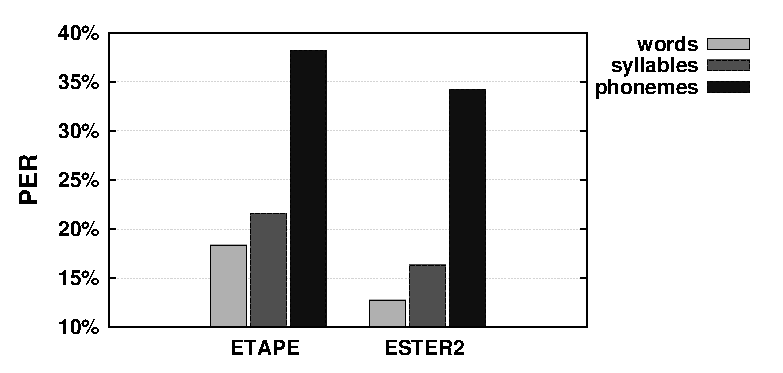
\includegraphics[scale=0.63]{Image/bestResults_ETAPE_ESTER}
\par\end{centering}

\caption{Summary of the results}
\label{Fig:performance}

\end{figure}


Figure \ref{Fig:performance} displays a summary of the results obtained
on both corpora. Given that ESTER2 contains mainly prepared speech
and that ETAPE contains mainly spontaneous speech, the results obtained
on ESTER2 are, as expected, better than the ones obtained on ETAPE.


\section{Conclusions}

This paper presented a detailed study on the phonetic decoding performance
of various modules on two French speech corpora (ETAPE and ESTER2).
We were interested in finding the best compromise between computational
cost and usability of results, constrains that must be met in order
to be able to create an embedded speech recognition decoder on a portable
terminal. The context is to later use such an approach as a support
for helping communication with deaf people.

Two baseline systems were considered. The first one relies on a large
vocabulary speech recognizer; it gives the best results (\textasciitilde{}18\%
phoneme error rate (PER) on ETAPE and \textasciitilde{}12\% PER on
ESTER2), but it uses a lot of memory and computational power. The
second one relies on a phonetic n-gram language model; it does not
use much memory, nor computational power, but it does not give good
results neither (\textasciitilde{}38\% PER on ETAPE and \textasciitilde{}34\%
PER on ESTER2).

Then syllable-based lexicons and associated 3-gram language models
were investigated. The lexicons of syllables and pseudo-syllables
were filtered according to the number of occurrences in the training
data and the number of phonemes. Keeping only the most frequent syllables
leads to a limited-size lexicon and language model, which nevertheless
provides good phonetic decoding performance. The phone error rate
is only 4\% worse (absolute) than the phone error rate obtained with
the large vocabulary recognizer, and much better than the phone error
rate obtained with the phone n-gram language model.

Future work will focus on the best, suitable way of presenting the
recognized information (phonemes, syllables, words or combinations),
based on relevant confidence measures, so that it maximizes communication
efficiency with deaf people.


\section{Acknowledgements}

The work presented in this article is part of the RAPSODIE project
(http://erocca.com/rapsodie).

\newpage{}


\begin{thebibliography}{10}
\bibitem[1]{IS1} Sch�nb�chler, J., ``Le traitement de la parole
pour les personnes handicap�es'', travail de s�minaire, Fribourg,
2003.

\bibitem[2]{IS2} Sokol, R., ``R�seaux neuro-flous et reconnaissance
de traits phon�tiques pour l'aide � la lecture labiale'', Th�se Universit�
de Rennes, 1996. 

\bibitem[3]{IS3}Cox, S., Lincoln, M., Tryggvason, J., Nakisa, M.,
Wells, M., Tutt, M. and Abbott, S., ``Tessa, a system to aid communication
with deaf people'', Proc. Assets'02, Vth Int. ACM Conf. on Assistive
Technologies, pp. 205-212, 2002.

\bibitem[4]{IS4} Woodcock, K., ``Ergonomics and automatic speech
recognition applications for deaf and hard-of-hearing users'', Technology
and Disability, vol. 7, pp. 147-164, 1997.

\bibitem[5]{IS5}Lippmann, R., ``Speech recognition by machines and
humans'', Speech Communication, n\textdegree{} 22, pp. 1-15, 1997.

\bibitem[6]{IS6}Coursant-Moreau, A. and Destombes, F., ``LIPCOM,
prototype d'aide automatique � la r�ception de la parole par les personnes
sourdes'', Glossa, n\textdegree{} 68, pp. 36-40, 1999.

\bibitem[7]{IS7}Jiang, H., ``Confidence measures for speech recognition:
A survey'', Speech Communication, vol. 45, n\textdegree{} 4, pp.
455-470, 2005.

\bibitem[8]{IS8}Razik, J., Mella, O., Fohr, D. and Haton, J.-P.,
``Transcription automatique pour malentendants : am�lioration � l'aide
de mesures de confiance locales'', Journ�es d'Etude de la parole,
2008.

\bibitem[9]{IS9}Zhang, L. and Edmondson, W. H., ``Speech recognition
using syllable patterns'', 7th International Conference on Spoken
Language Processing, 2002.

\bibitem[10]{IS10}Tachbelie, M., Besacier, L. and Rossato, S., \textquotedblleft{}Comparison
of syllable and triphone based speech recognition for Amharic\textquotedblright{},
Proceedings of the LTC 2011, pp. 207\textendash{}211, 2011.

\bibitem[11]{IS11} Ganapathiraju, A., Hamaker, J., Ordowski, M.,
Doddington, G. and Picone, J., ``Syllable-based large vocabulary
continuous speech recognition'', IEEE Transactions on Speech and
Audio Processing., vol. 9, no. 4, pp. 358\textendash{}366, 2001.

\bibitem[12]{IS12} H�m�l�inen, A., Boves, L. and de Veth, J., ``Syllable-Length
Acoustic Units in Large-Vocabulary Continuous Speech Recognition'',
Proceedings of SPECOM, 2005.

\bibitem[13]{IS13}Blouch, O., Collen, P., ``Reconnaissance automatique
de phonemes guide par les syllables'', Journ�es d'Etude de la parole,
2006.

\bibitem[14]{IS14}Rastrow, A., Sethy, A., Ramabhadran, B. and Jelinek,
F., ''Towards using hybrid, word, and fragment units for vocabulary
independent LVCSR systems'', Proceedings Interspeech'2009, 2009. 

\bibitem[15]{IS15}Bigi, B., Meunier, C., Bertrand, R. and Nesterenko,
I. ``Annotation automatique en syllabes d\textquoteright{}un dialogue
oral spontan�'', Journ�es d'Etude de la parole, 2010.

\bibitem[16]{IS17}Galliano, S., Gravier, G. and Chaubard, L., ``The
ESTER 2 evaluation campaign for rich transcription of French broadcasts'',
Proceedings INTERSPEECH'2009, 2009. 

\bibitem[17]{IS18}Gravier, G., Adda, G., Paulson, N., Carre, M.,
Giraudel, A. and Galibert, O., ``The ETAPE corpus for the evaluation
of speech-based TV content processing in the French language'', 8th
International Conference on Language Resources, Evaluation and Corpora,
2012.

\bibitem[18]{IS19}Est�ve, Y., Bazillon, T., Antoine, J., B�chet,
F. and Farinas, J., ``The EPAC corpus: Manual and automatic annotations
of conversational speech in French broadcast news'', in Proc. LREC\textquoteright{}2010,
European conference on Language Resources and Evaluation, 2010.

\bibitem[19]{IS20}Mendon�a, �., Graff, D., DiPersio, D., ``French
gigaword third edition'', Linguistic Data Consortium, 2011.

\bibitem[20]{IS21}M. de Calm�s, and G. P�rennou, ``BDLEX : a Lexicon
for Spoken and Written French'', Language Resources and Evaluation,
pp.1129-1136, 1998. 

\bibitem[21]{IS22}Illina, I., Fohr, D. and Jouvet, D., ``Grapheme-to-Phoneme
Conversion using Conditional Random Fields'', Proceedings INTERSPEECH'2011,
2011. 

\bibitem[22]{IS23}Stolcke, A., ``SRILM an Extensible Language Modeling
Toolkit'', 7th International Conference on Spoken Language Processing,
2002.

\bibitem[23]{IS24} Placeway, P., Chen, S., Eskenazi, M., Jain, U.,
Parikh, V., Raj, B., Ravishankar, M., Rosenfeld, R., Seymore, K.,
Siegler, M., Stern, R. and Thayer, E., ``The 1996 Hub-4 Sphinx-3
System'', Carnegie Mellon University, 1996.

\bibitem[24]{IS25}Fohr, D. and Mella, O., ``CoALT: A Software for
Comparing Automatic Labelling Tools'', Language Resources and Evaluation,
2012.\end{thebibliography}

\end{document}
